\chapter{Visualize spectral distances}
\label{ch:visualize-spectral-distances}

\begin{wrapfigure}{o}{0.65\textwidth}
	\vspace{-1.5 cm}
    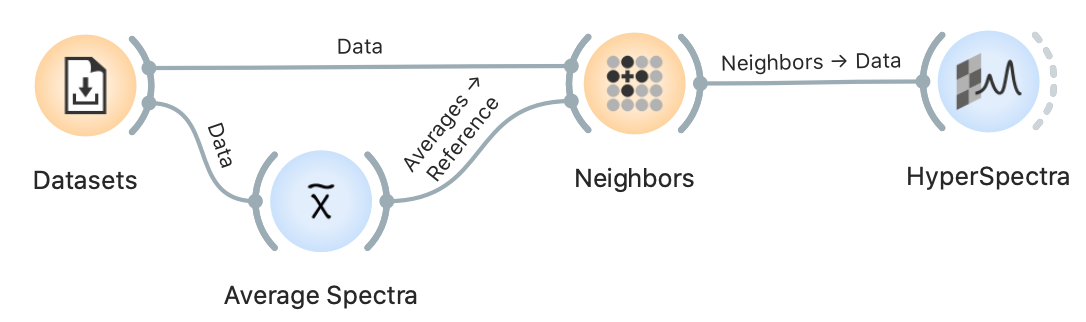
\includegraphics[scale=0.6]{graphics/ch-visualize_spectral_distances/ch-visualize_spectral_distances-fig1.png}
\end{wrapfigure}

Let's consider a spectrum, or any other data entry for that matter, as a point in a multidimensional space. We can define distance metrics between these points and visualize the distance values from one another or from a selected reference point or reference spectrum. By doing so, we can explore how similar our measurements are to a selected reference. We can do this on a series of spectra or even on hyperspectral maps!

If you build the workflow shown above this paragraph in \mutation\ you will be able to explore various distance metrics. First, let's use the \textit{'Liver cirrhosis - spectral image'} dataset provided by the \widget{Datasets} widget, then calculate the \textit{Euclidean distances} from the average spectrum with the \widget{Neighbors} widget and visualize them in \widget{Hyperspectra}. 

\medskip
Can you reproduce the results below? Pay attention to the color scheme.

\begin{figure*}[h]
\centering
\infinitewidthbox{
  \stackinset{r}{-0.5\linewidth}{t}{+0.1\linewidth}
  {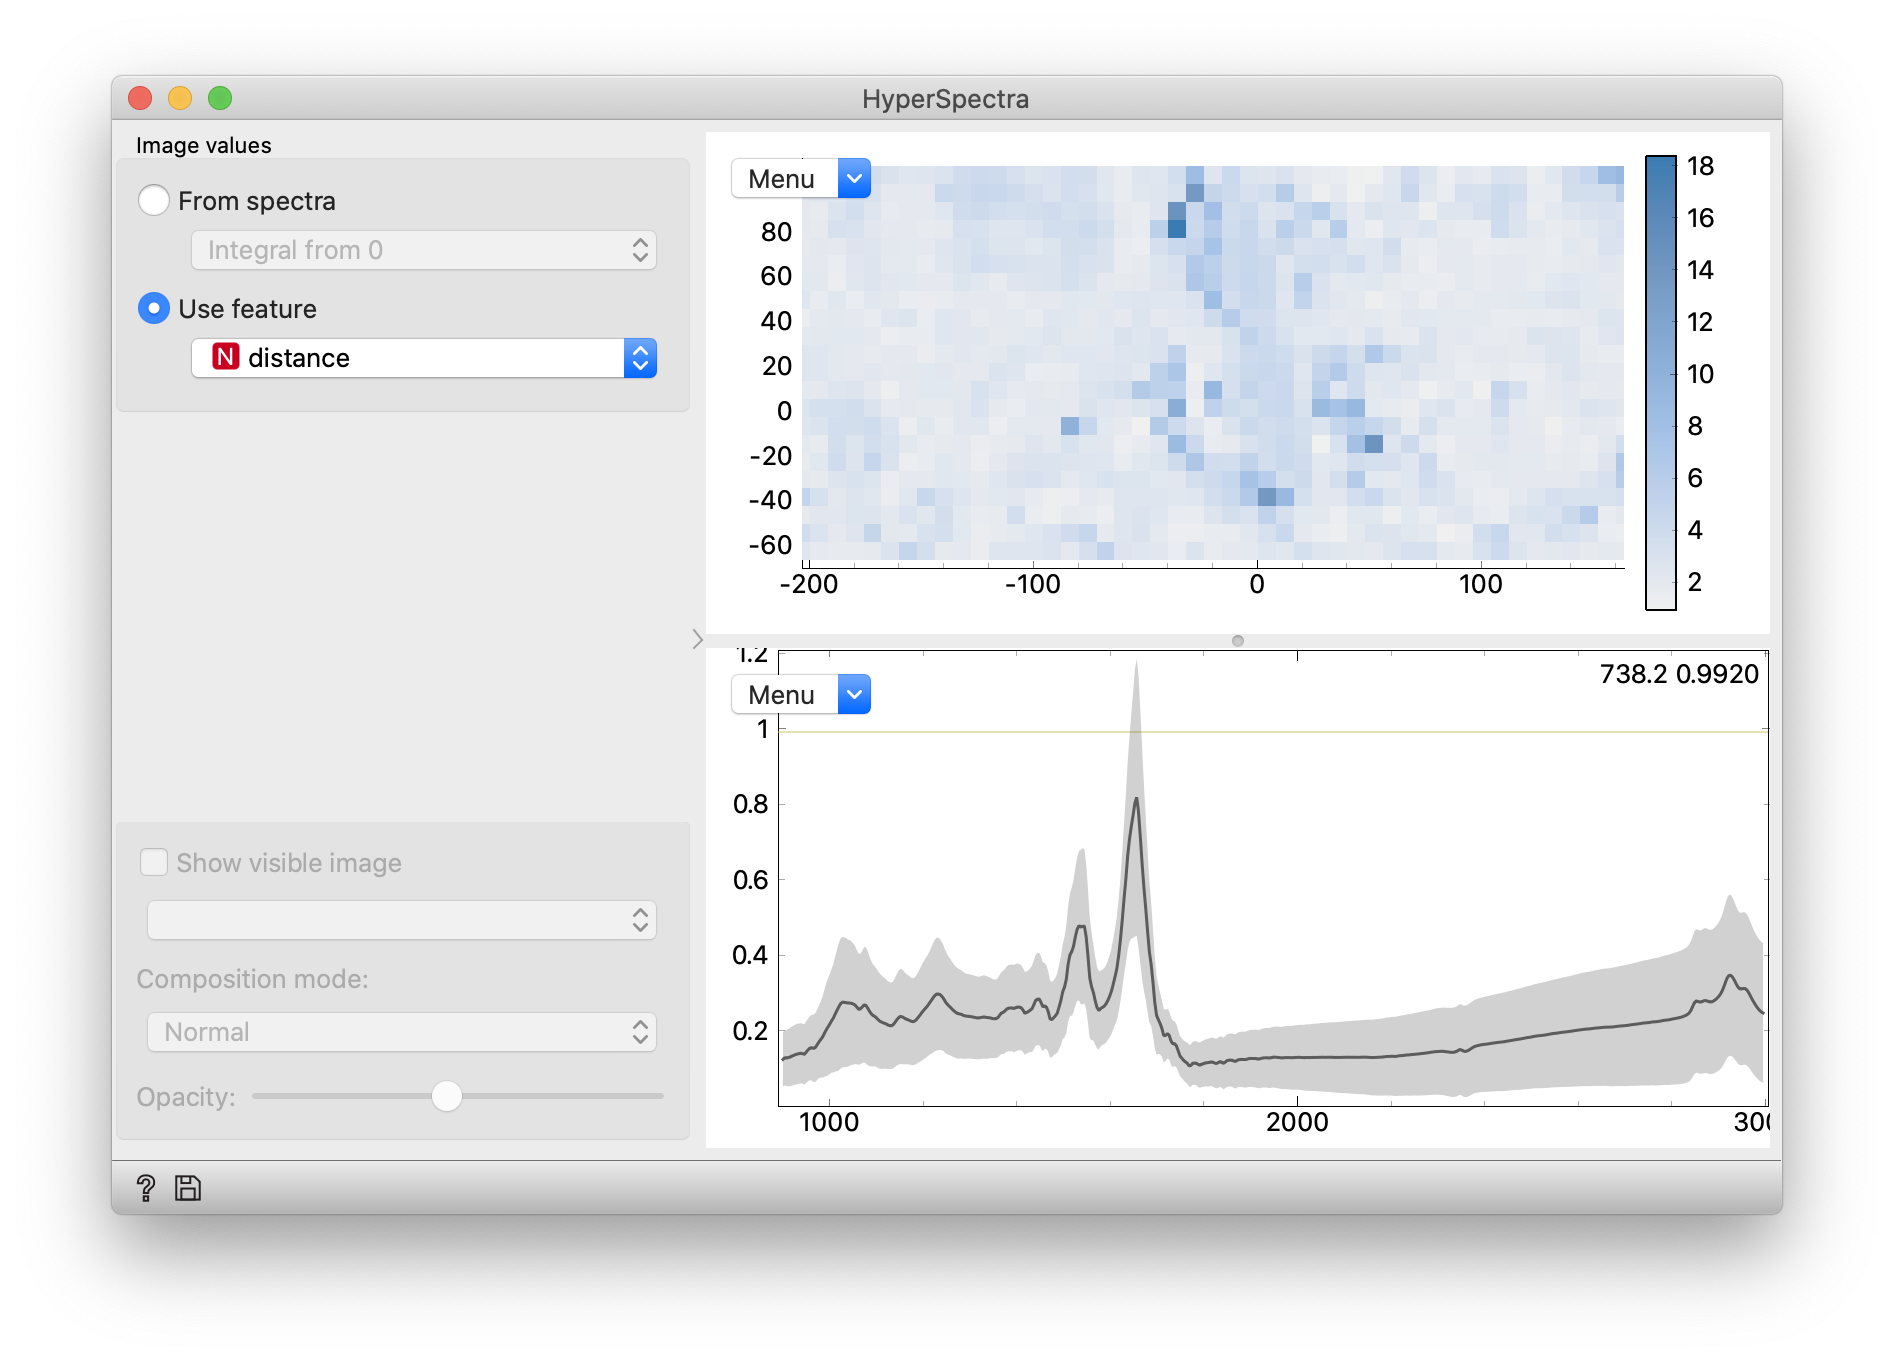
\includegraphics[scale=0.4]{graphics/ch-visualize_spectral_distances/ch-visualize_spectral_distances-fig3.png}}
  {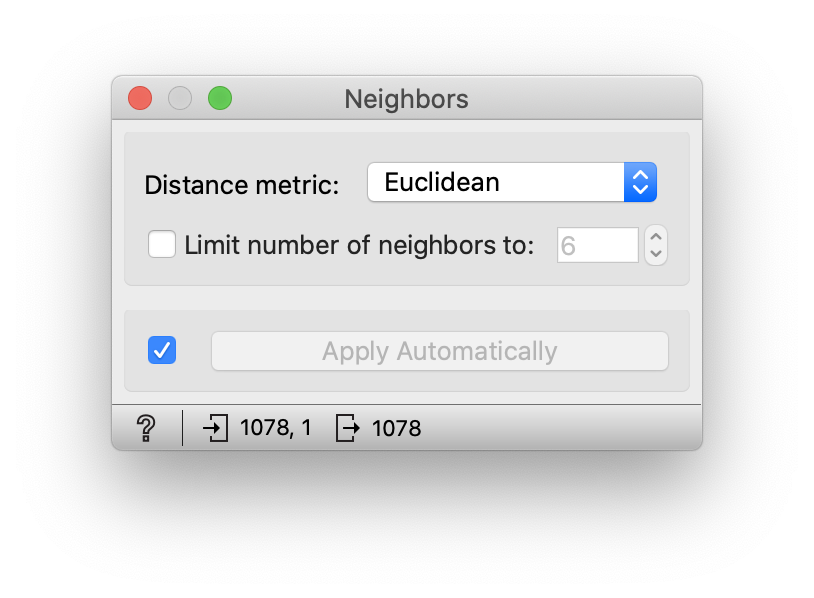
\includegraphics[scale=0.6]{graphics/ch-visualize_spectral_distances/ch-visualize_spectral_distances-fig2.png}}
  \hspace{8cm}
  }
%\caption{Try changing the parameters!}

\end{figure*}

Explore different distance metrics, inspect distances in a \widget{Data Table} widget. Don't forget, you can select points on the top map and see the corresponding spectra on the bottom in \widget{Hyperspectra}. 

% I would like to have a special environment called notes for example that we can switch on or off to print or hide lecturer notes.
\lecnotes{Possibility for discussion of the general mathematical properties of distance functions. See \url{https://en.wikipedia.org/wiki/Metric_(mathematics)}}